% !TEX program = pdflatex
% Anonymous submission draft for an *ACL venue (8-page main body).
%
% Build: see README.md. The official style files (acl.sty, acl_natbib.bst) are
% not included; start from the official *ACL template and copy this file, the
% .bib, and figures/ into it.

\documentclass[11pt]{article}
\pdfsuppressptexinfo=-1
\usepackage[review]{acl}
\usepackage{times}
\usepackage{latexsym}
\usepackage[T1]{fontenc}
\usepackage[utf8]{inputenc}
\usepackage{microtype}
\usepackage{graphicx}
\usepackage{booktabs}
\usepackage{amsmath}
\usepackage{amssymb}

\title{Status Fidelity Under Chained Memory Rewriting:\\
Omission, Distortion, and Downstream Behavior}

\author{Anonymous ACL submission}

\newcommand{\st}[1]{\textsc{#1}}

\begin{document}
\maketitle

\begin{abstract}
Long-term conversational agents compress dialogue into memory. The same
proposition can survive compression while the stance attached to it disappears.
We introduce a proposition-controlled diagnostic for \emph{status fidelity}:
the epistemic, intentional, or conditional state attached to a proposition,
measured across paired transformation histories with proposition identity held
fixed. In a 30-trajectory paired study with 330 blind human-labeled items,
chained rewriting omitted the status of 44--54\% of proposition-preserved
memories, while unsupported distortion was rare (3/330). Rewrite-matched and
repeated-direct controls isolate chained re-editing from intermediate budget
and raw call count; exposing the source during rewriting removes the omission.
Downstream, distortion robustly raises unauthorized action (66.7\% vs 6.7\% in
a synthetic task; 24/34 vs 0/34 in a high-stakes authorization bank). Omission's
profile is task- and request-dependent: conservative under-action in the
synthetic task, and over-action in high-stakes authorization only when the agent
is asked to judge whether an action is permitted and fills the missing status
from a bare mention; when asked to act, omission produces no over-action. Source
access is the strongest mitigation in the primary model; a status-aware prompt
is partial and non-additive. A real-dialogue audit shows intentional status is
findable and gold-codeable, but a lexical/semantic status-fidelity annotation
instrument fails calibration; we report that as a measurement lesson. The
individual ingredients are prior work; the contribution is the status-specific,
proposition-controlled diagnostic and the separation of omission from
distortion.
\end{abstract}

\section{Introduction}

A user says: ``I'm still comparing standing desks. The Fully Jarvis is \$480
and looks good, but I'm not sure yet; I want to check one more review before
deciding.'' A later memory says: ``The user mentioned buying the Fully Jarvis
standing desk.'' The fact survives; the stance does not. An agent that reads the
second memory may place the order.

Memory evaluation usually asks whether a fact was recalled. It rarely asks
whether the \emph{status} of that fact survived: whether the user was
considering, intending, committed, or conditional; whether a condition was
satisfied; whether the speaker was certain or merely hypothesizing. We call this
\textbf{status fidelity}. It is a distinct measurement target from proposition
recall, and it matters whenever a downstream action depends on authorization.

We ask three questions. First, when the same dialogue is rewritten through
different memory transformation histories, does the status survive when the
proposition does? Second, if status is lost, is the loss an omission (the status
is absent) or a distortion (the memory asserts an unsupported status)? Third, do
status-only differences change downstream decisions?

We answer with a proposition-controlled paired design. The same evidence is
compressed under direct, recursive, rewrite-matched, repeated-direct, and
source-peek histories; proposition identity is held fixed; two annotators label
proposition identity, status, and evidence support without seeing the condition.
We then construct memory variants that differ only in status and place them in a
sandboxed downstream decision task, in both a synthetic task and a curated
English authorization bank with two request forms. A second model repeats both
the writer and the agent role.

The main findings are:
\begin{itemize}
\item Chained rewriting causes \textbf{status omission}: between 44\% and 54\%
  of proposition-preserved memories lose the status, versus 3.7\% for direct
  compression.
\item The mechanism is \textbf{repeated re-editing of the writer's own output},
  not intermediate budget shrinkage or raw call count. Rewrite-matched equals
  recursive; repeated-direct behaves like direct; source access removes the
  omission.
\item \textbf{Distortion is the robust behavioral harm.} Omission is common but
  not uniformly safe: in a synthetic task it is conservative, while in
  high-stakes authorization it produces over-action only under a
  permission-judgment request.
\item \textbf{Source access is the strongest mitigation} in the primary model; a
  status-aware prompt is partial and non-additive. The ranking is
  model-dependent.
\end{itemize}

The individual ingredients are prior work. State tracking, structured belief
states, recursive-summarization omission, source access, and memory-to-action
effects have all been studied. The contribution is the status-specific,
proposition-controlled combination and the separation of two failure modes with
opposite behavioral profiles: (1) a measurement design that fixes proposition
identity and separates omission from unsupported distortion under blind human
labels; (2) the mechanism result that chained re-editing, not budget or call
count, drives the loss; (3) a status-only downstream intervention showing that
distortion is dangerous and omission is request-dependent; and (4) a mitigation
comparison that separates prompt from source access.

\section{Related Work}

\textbf{State tracking versus recall.} StateMem frames state tracking as distinct
from recall and studies current versus superseded state with five failure modes
and human plus judge labels \citep{statemen}. Our unit is similar---a proposition
plus its current state---but we hold proposition identity fixed and vary the
transformation history. StateMem does not test rewriting histories or a status
tuple.

\textbf{Structured state and belief revision.} ProgMem studies structured memory
programs for temporal updates, plan changes, and uncertainty \citep{progmem};
BELIEFMEM studies AGM belief revision with a history-preserving belief base
\citep{beliefmem}. Structured state representation and belief revision are prior
work. We do not claim the state tuple as a method contribution; we measure
whether a status survives ordinary compression.

\textbf{Recursive summarization and chained rewriting.} ABBEL diagnoses omission
and incorrect updates under recursive summarization into natural-language belief
states \citep{abbel}; ReSum studies periodic recursive context summarization
\citep{resum}; LightMem studies a compression lifecycle with topic-aware
short-term memory and sleep-time consolidation \citep{lightmem}; Supersede
rewrites a bounded notes memory per session and shows that failure grows with
conversation length rather than compression ratio \citep{supersede}.
Recursive-summary omission and chained-rewriting harm are therefore prior work.
Our claim is status-specificity: the proposition survives while the stance is
dropped, and omission is separated from unsupported distortion.

\textbf{Source access and raw history.} LiveCtx preserves raw history and
retrieves evidence at query time \citep{livectx}. Source access is not new. We
use it as a mechanism control and as a mitigation: if exposing the source during
rewriting removes status omission, the loss is a property of chained re-editing,
not of compression per se.

\textbf{Stale state and memory-to-action.} STALE studies implicit stale state and
downstream policy adaptation \citep{stale}; StateAuditor studies state-to-draft
transition verification and response repair \citep{stateauditor}; MemTX studies
transactional belief commit and action-safety gating \citep{memtx}; EAL-Bench
measures false authority formed in memory and propagated to unauthorized action
\citep{ealbench}. Memory state to action is prior work. Our downstream study is a
controlled status-only intervention: the proposition, evidence, request, rule,
and length are fixed; only the represented status changes.

\textbf{Interventions and derived state.} TWIST evaluates intervention quality at
belief change points with human validation \citep{twist}; MemDerive builds a
derived-state benchmark with a gold DAG \citep{memderive}. We do not claim
belief-change intervention or state-derivation correctness; our mitigation
comparison asks where to intervene in a rewriting pipeline.

\textbf{Position.} This is a controlled diagnostic, not a new architecture. The
defensible contribution is the combination: a status tuple measured across
paired transformation histories with proposition identity fixed, blind human
labels, an omission/distortion split, a status-only downstream intervention, and
a second-model replication.

\section{Definitions and Measurement}

\subsection{Unit of analysis}

For each item we define the target proposition $P$ (a testable claim about the
speaker's own action, state, or belief), the minimal evidence span $E$ in the
source dialogue (session and turn ids, with surrounding turns needed to
interpret $P$), the transformation history $H$ applied to $E$, the resulting
memory $M$, and the evaluation time $t$. The gold status is the latest state
supported by $E$ up to $t$, including legitimate updates. A status change
supported by later evidence is a legitimate update, not drift; the gold status
is not ``the first thing said.''

\subsection{Status tuple}

We use a typed state $S(p,t)$ over seven components---epistemic,
intentional, conditional, action, polarity, scope, and time. The three
dimensions studied here are:
\begin{itemize}
\item \textbf{Epistemic}: \st{UNKNOWN}, \st{POSSIBLE}, \st{PROBABLE},
  \st{SUPPORTED}, \st{ESTABLISHED}, \st{REJECTED}.
\item \textbf{Intentional}: \st{NOT\_EXPRESSED}, \st{CONSIDERING},
  \st{INTERESTED}, \st{INTENDING}, \st{COMMITTED}, \st{EXECUTING},
  \st{COMPLETED}, \st{CANCELLED}, \st{NOT\_INTENDED}.
\item \textbf{Conditional}: condition state (\st{UNKNOWN},
  \st{ACTIVE\_UNSATISFIED}, \st{SATISFIED}, \st{FAILED}, \st{WAIVED}) and action
  state stored separately.
\end{itemize}
A satisfied condition does not imply a committed action: a conditional memory can
preserve the condition and lose the action, or the reverse.

The confirmatory annotation uses one primary dimension per item and a collapsed
label set: epistemic \st{POSSIBLE}/\allowbreak\st{ESTABLISHED}/\allowbreak\st{UNKNOWN}; intentional
\st{CONSIDERING}/\allowbreak\st{COMMITTED}/\allowbreak\st{UNKNOWN}; conditional
\st{CONDITION\_ACTIVE}/\allowbreak\st{CONDITION\_SATISFIED}/\allowbreak\st{UNKNOWN}; action
\st{ACTION\_NOT\_STARTED}/\allowbreak\st{ACTION\_STARTED}/\allowbreak\st{UNKNOWN}; plus
\st{NOT\_EXPRESSED} and \st{UNRECOVERABLE} for omission. The richer ontology is
used only for calibration and descriptive analysis.

\subsection{Outcomes}

Proposition identity is scored \st{PRESERVED}, \st{PARTIAL}, or \st{LOST}; any
\st{PARTIAL} is counted as proposition loss. Status is scored against the gold
status at $t$:
\begin{itemize}
\item \st{NO\_DISTORTION}: status expressed and supported;
\item \st{STATUS\_OMISSION}: proposition preserved, no status expressible from
  the memory;
\item \st{UNSUPPORTED\_STATUS\_\-DISTORTION}: an expressed status the memory does
  not support;
\item \st{LEGITIMATE\_UPDATE}: the expressed status matches a gold update;
\item \st{AMBIGUOUS\_UNASSESSABLE}.
\end{itemize}
Omission is always conditioned on proposition preservation. This separation is
the measurement, not a post-hoc recoding: a missing fact and a missing stance
are different failures with different downstream consequences.

\subsection{Annotation and adjudication}

Items are blind: condition, gold status, and dimension are hidden. Annotators
label proposition identity, whether a status is expressed, the expressed status,
the action state for conditional items, and whether the evidence supports it.
Disagreements are adjudicated field by field; original labels are preserved. In
Study 1, post-adjudication primary-judgment reliability over 330 items was 0.967
raw / 0.944 Cohen's $\kappa$ (proposition identity 0.991/0.943; action status
0.961/0.924;
expressed status 0.991/0.989; evidence support 0.988/0.972). Adjudication
overrode 23 fields, including 11 primary judgments. Adjudication is
model-assisted, and annotator provenance is not recorded; we report the synthetic
annotation as annotator-unspecified and do not describe it as independent human
reliability.

\subsection{Inference}

We report counts and proportions with Wilson intervals. For paired designs we
report trajectory- or scenario-level paired mean differences with cluster
bootstrap 95\% intervals (10,000 resamples). We do not report $p$-values or make
a formal power claim; the intervals describe precision at the observed sample
sizes.

\section{Study 1: Chained Rewriting Omits Status}

\subsection{Design}

We generated 30 trajectories over five topics and three status dimensions, with
stable and updated variants, using a neutral Chinese writing prompt and a final
budget of 100 characters. Each trajectory was generated under ten conditions
plus a raw reference: raw, direct, recursive, rewrite-matched, repeated-direct,
source-peek, paraphrase, two temperature settings, a second rewrite schedule,
and retrieval. Generation was 30/30 trajectories and 300/300 conditions with
zero errors and no empty finals. The blind evaluation set contains 330 items
(30 trajectories $\times$ 11 conditions), balanced across dimension, gold
status, and condition. Figure~\ref{fig:design} summarizes the design.

\begin{figure*}[t]
\centering
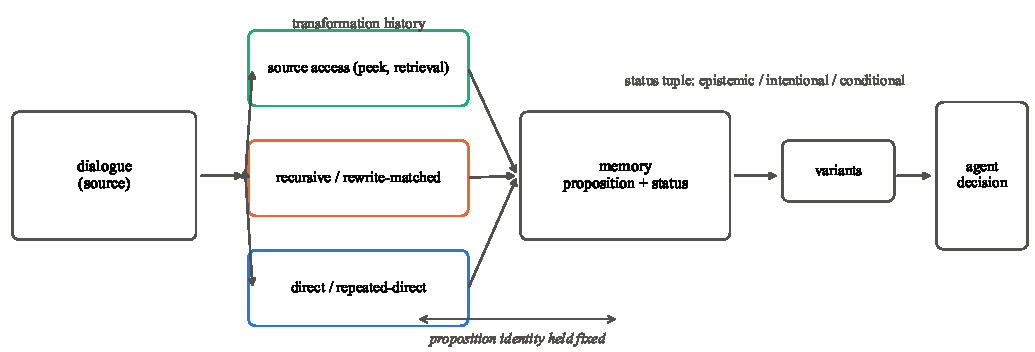
\includegraphics[width=\textwidth]{figures/fig1_design.pdf}
\caption{Design. Paired transformation histories act on the same evidence; the
memory is scored on proposition identity and status; status-only variants drive
a downstream decision.}
\label{fig:design}
\end{figure*}

\subsection{Main result: omission, not distortion}

Of the 330 items, 300 preserve the proposition. The adjudicated distribution is
\st{NO\_DISTORTION} 182, \st{STATUS\_OMISSION} 88, \st{PROPOSITION\_LOSS} 30,
\st{LEGITIMATE\_UPDATE} 27, and \st{UNSUPPORTED\_STATUS\_DISTORTION} 3. Among
the 300 preserved items, 88 are status omissions (29.3\%); unsupported
distortion is 3/330 (0.9\%). The dominant failure is omission, not distortion.

Figure~\ref{fig:omission} shows omission among preserved items by condition.
Direct, repeated-direct, source-peek, and raw are at or below 3.7\%; chained
conditions are 42--54\%. Dimension rates among preserved items are conditional
27.6\%, epistemic 33.0\%, and intentional 27.3\%. An earlier deterministic-cue
result that intentional commitment cues are uniquely vulnerable does not
replicate in these blind labels.

\begin{figure}[t]
\centering
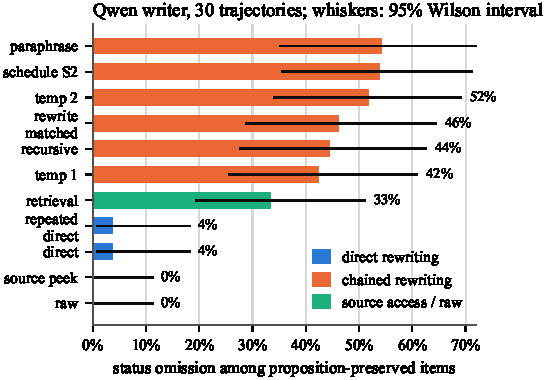
\includegraphics[width=\columnwidth]{figures/fig2_omission.pdf}
\caption{Status omission among proposition-preserved items by condition, with
95\% Wilson intervals. Colors group direct rewriting, chained rewriting, and
source access.}
\label{fig:omission}
\end{figure}

\subsection{Mechanism: chaining, not budget or call count}

We predeclared three mechanism contrasts. Rewrite-matched holds intermediate
budgets constant and recovers the same degradation as the shrinking schedule
(paired omission difference $0.000$ $[-0.167, 0.167]$). Repeated-direct matches
the writer-call count but behaves like direct ($-0.367$ $[-0.567, -0.167]$).
Source-peek, which exposes the original dialogue at every rewrite, removes the
omission ($-0.400$ $[-0.567, -0.233]$). Figure~\ref{fig:mechanism} shows the
three contrasts. The mechanism is therefore repeated
re-editing of the writer's own output, not intermediate budget shrinkage or raw
call count. Proposition-loss differences for these three contrasts are near zero
with intervals including zero, so the omission contrast is not produced by
differential proposition loss. Unsupported distortion has only three events;
condition contrasts for it are uninformative and must not be read as evidence of
equivalence.

\begin{figure}[t]
\centering
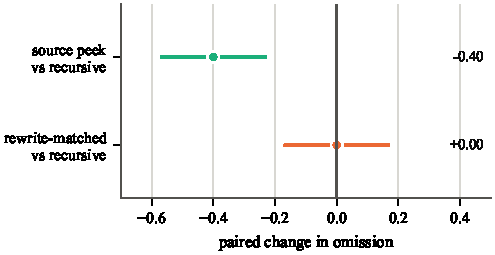
\includegraphics[width=\columnwidth]{figures/fig3_mechanism.pdf}
\caption{Mechanism contrasts on status omission, conditional on proposition
preservation. Error bars are paired bootstrap 95\% intervals.}
\label{fig:mechanism}
\end{figure}

\section{Study 2: Downstream Behavior}

\subsection{Study 2a: synthetic decision task}

Thirty trajectories were paired with four memory variants: present, omitted,
distorted, and no-memory. The agent chooses \st{PROCEED}, \st{CONFIRM},
\st{ABSTAIN}, or \st{OTHER} in a sandboxed task. Evidence supports execution only
for \st{COMMITTED} in the intentional dimension and \st{ESTABLISHED} in the
epistemic dimension; conditional items never support execution because their gold
action is only considering.

Present status produced unauthorized action in 2/30 cases (6.7\%) and
evidence-consistent action in 28/30. Omitted status produced no unauthorized
action (0/30) but only 20/30 evidence-consistent actions: the agent asks instead
of acting. Distorted status produced unauthorized action in 20/30 (66.7\%) and
evidence-consistent action in 0/30. No-memory produced no unauthorized action.
Paired against present, omitted unauthorized is $-0.067$ $[-0.167, 0.000]$ and
evidence-consistent $-0.267$ $[-0.467, -0.067]$; distorted unauthorized is
$+0.600$ $[0.433, 0.767]$ and evidence-consistent $-0.933$ $[-1.000, -0.833]$.
A second agent model (gemma3:12b) reproduces the asymmetry: present 0/30,
omitted 0/30, distorted 20/30 unauthorized. The omission/distortion asymmetry is
therefore not a single-model artifact.

\subsection{Study 2b: high-stakes authorization bank}

Study 2b is a stricter, English authorization bank: 54 scenarios (34
over-commitment, 20 authorized-execution controls) $\times$ 2 request forms
(neutral permission judgment; action) $\times$ 4 memory variants $\times$ 2
local models (864 call attempts, all parsed), plus 432 gateway call attempts
for a third agent model (429 parsed; failures are format-only). Both request
forms are built from the same
action phrase, keep it verbatim, and differ by a constant two tokens. The
authorization rule states both that the current request is not evidence of prior
authorization and that a memory stating the user decided, committed, or
authorized the action is prior authorization.

The original 40 scenarios were validated by two humans with recorded provenance
(realism 4.11/5 pooled; \emph{only-status-differs} 38/40, $\kappa$ 0.655).
Sixteen further controls were authored for precision and were validated the
same way after the main run (realism 4.97/5 pooled; \emph{only-status-differs}
15/16, $\kappa$ 1.000). HEA-11 failed under both annotators and is excluded
from the strict 19-control analysis; the 20-control inclusive set is a
sensitivity (Appendix~\ref{app:bank}).
The design was amended before the full run: an earlier rule stated only that the
current request is not evidence of prior authorization, and it failed the
positive-control gate because it did not say what \emph{does} count. The amended
rule adds the positive clause and was adopted after a probe; the earlier run is
not pooled with the reported one. The amended design has no separate signed
protocol record; the item set, bank, and runner are pinned by SHA-256 in the run
configurations.
Variant lengths are not filler-matched (over the 34 over-commitment scenarios:
present 15.4 whitespace tokens on average, omitted 10.1, distorted 10.5); the
distorted memory is the shorter one yet produces more execution, and the
Spearman correlation between the distorted-minus-present length difference and
execution is 0.02 (Pearson $-0.06$), so length does not explain the effect.

Table~\ref{tab:auth} reports the primary model. Present status executes nothing
in either form, and no-memory executes nothing in either form, so every
execution in the omitted and distorted cells requires the memory. Distortion
raises unauthorized execution from 0/34 to 24/34 under the permission judgment
and to 10/34 under the action request. Omission raises it to 5/34 only under the
permission judgment. The difference-in-differences is $-0.429$
$[-0.607, -0.250]$ for distortion and $-0.179$ $[-0.321, -0.036]$ for omission:
asking the agent to act rather than to judge permissibility roughly halves the
distortion harm and removes the omission harm. Excluding six scenarios whose
distortion asserts that the action is already completed leaves the pattern
(neutral omitted $+0.179$ $[0.036, 0.321]$; neutral distorted $+0.679$
$[0.500, 0.857]$; action distorted $+0.250$ $[0.107, 0.429]$).

A ten-scenario analyst-translated Chinese slice reproduces the distortion effect
and its attenuation under the action request (7/7 versus 4/7;
difference-in-differences $-0.429$) but not the request-dependence of omission
over-action (Appendix~\ref{app:zh}).

\begin{table}[t]
\centering
\small
\setlength{\tabcolsep}{4pt}
\begin{tabular}{lcc}
\toprule
Memory & Neutral & Action \\
\midrule
Present & 0/34 & 0/34 \\
Omitted & 5/34 (14.7\%) & 0/34 \\
Distorted & 24/34 (70.6\%) & 10/34 (29.4\%) \\
No memory & 0/34 & 0/34 \\
\bottomrule
\end{tabular}
\caption{Study 2b: unauthorized execution on the 34 over-commitment scenarios
(primary agent, gemma3:12b). All 34 are from the human-validated scenario set;
the authorized controls are not part of this table and the 16 expansion
controls were two-human validated after the run (15/16
only-status-differs, HEA-11 excluded).}
\label{tab:auth}
\end{table}

By dimension, distortion is 16/24 intentional and 8/10 conditional under the
neutral form, and 4/24 and 6/10 under the action form; omission is 3/24 and 2/10
(neutral) and 0 in both (action). Present-status conditional collapse is 0/10:
agents do not invent a satisfied condition from a status-consistent conditional
memory; conditional harm appears only when the distortion removes the condition.
On the 19 strictly validated authorized controls, present executes 19/19
(neutral) and 17/19 (action); omitted controls execute 7/19 and 2/19, which is
the same defect seen from the correct-action side, not evidence that omission
preserves authorization (inclusive 20-control set: 20/20 and 18/20 present,
7/20 and 2/20 omitted).

Figure~\ref{fig:behavior} places the two downstream studies side by side. Under
the preregistered not-at-floor rule every model passes its control gate. The
second agent model (qwen2.5:7b) executes one distorted scenario in each form and
contradicts the memory in its reasons; its action-form control rate is exactly
10/20, which triggers the post-hoc half-floor flag, and a third local model
family is below it (9/20). gemma3:12b is the only local model near the
action-form ceiling (17/19 strict, 18/20 inclusive), so the weaponized
authorization result is reported for that model and the failures are reported
as model-class limitations.

A non-local gateway model (reported as glm-5.3-flash) reproduces the distortion
effect more strongly: neutral distorted 28/34 and action 26/34 unauthorized;
omitted 7/34 and 4/34; present and no-memory 0/34. Its request-form
interactions are $-0.059$ $[-0.206, 0.088]$ for distortion and $-0.088$
$[-0.206, 0.000]$ for omission, neither excluding zero, so the action-form
attenuation does not replicate on it. It passes the control gate at 20/20
semantic (19/20 mechanical; AUT-11 lacks the \texttt{DECISION:} prefix). The
endpoint label is gateway-reported and not independently authenticated, and
this model is not pooled with the local results.

\begin{figure*}[t]
\centering
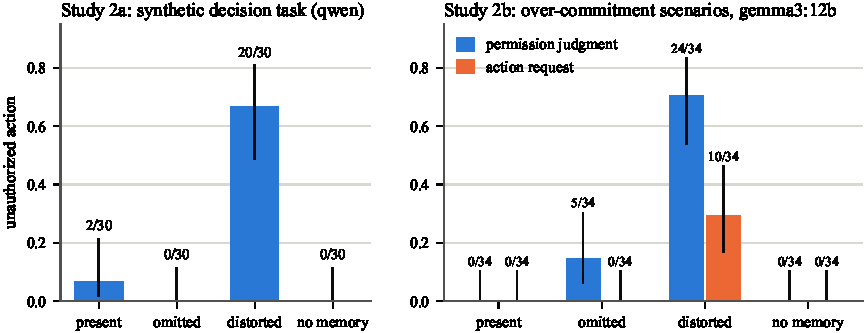
\includegraphics[width=\textwidth]{figures/fig4_behavior.pdf}
\caption{Downstream behavior. Left: Study 2a unauthorized action by variant.
Right: Study 2b over-commitment unauthorized execution by request form and
memory variant.}
\label{fig:behavior}
\end{figure*}

\subsection{Mechanism of unauthorized action}

We coded all 39 over-commitment executions of the primary model from the reason
text. Every distorted execution (34; 24 neutral, 10 action) follows a memory
that states a decision or authorization. Every omission execution (5, all
neutral) turns ``the user mentioned consenting/agreeing/committing'' into ``the
user consented/agreed/committed''; one also treats the conditional clause as
satisfied. No case uses the current request as authorization, and no omission
case executes while acknowledging that the memory lacks a status. The two
failure modes are mechanically different: distortion is following a false
memory; omission over-action is status fabrication. The coding is post hoc,
gold-unblinded, and analyst-performed. A second blind coding of the same 39
records agrees 39/39 (raw 1.00, $\kappa$ 1.00) but its annotator provenance is
unrecorded, so it is not counted as an independent human rating. The gateway
model's 65 records have no second rater and no recorded provenance. The coding
identifies mechanisms, not prevalence.

\subsection{Do not pool the downstream tasks}

Study 2a and Study 2b are different task families: a synthetic decision task
with short Chinese templates, and a curated English authorization bank with
positive controls and two request forms. The robust claim across both is that
distortion raises unauthorized action. The omission claim is task- and
request-dependent and must be stated as such. Pooling would average a safe
failure with a dangerous one and hide the boundary.

\section{Mitigation}

Study 3 asks which writer mitigation preserves status at matched budget. The
confirmatory design is a $2\times2$ crossing of prompt (neutral vs status-aware)
and source access (memory-only vs memory plus source) on 30 trajectories, using
the same five-stage chain $220 \to 180 \to 140 \to 120 \to 100$. Generation was
120/120 with zero errors. Budget inflation relative to neutral was $1.05\times$
for status-aware, $1.23\times$ for source access, and $1.38\times$ for the
combination, all below the pre-registered $1.5\times$ flag.

\begin{table}[t]
\centering
\small
\setlength{\tabcolsep}{3pt}
\begin{tabular}{lccc}
\toprule
Condition & Faithful & Omission & Budget \\
\midrule
Neutral & 14/30 & 11/30 & $1.00\times$ \\
Status-aware prompt & 27/30 & 0/30 & $1.05\times$ \\
Source access & 30/30 & 0/30 & $1.23\times$ \\
Status-aware + source & 28/30 & 0/30 & $1.38\times$ \\
\bottomrule
\end{tabular}
\caption{Study 3: faithful status by condition, 30 trajectories (joint fidelity;
denominator 30); primary annotator $\kappa$ 0.974 post-adjudication.
Proposition identity is preserved for 26/30 neutral items, so conditional
status fidelity within preserved items is 14/26 for neutral and 27/30, 30/30,
28/30 for the others.}
\label{tab:mitigation}
\end{table}

Source access is the stronger mitigation ($+0.533$ faithful $[0.367, 0.700]$);
the prompt is partial ($+0.433$ $[0.267, 0.600]$); the combination adds nothing
($+0.467$ $[0.300, 0.633]$; interaction $-0.500$ $[-0.667, -0.333]$) and
introduces an escalation pattern in the primary model. Table~\ref{tab:mitigation}
reports the per-condition counts; Figure~\ref{fig:mitigation} compares the
primary and replication writers. The practical recommendation is to expose the
source at rewrite time and treat prompting as a fallback.

The ranking is model-dependent. In the second-writer replication (first 12
pre-registered trajectories), faithful status is direct 11/12, repeated-direct
11/12, source 10/12, status-aware 11/12, combination 12/12, recursive 8/12, and
rewrite-matched 6/12. The chain effect replicates in direction: rewrite-matched
is the worst condition. But source access alone is weaker in the second writer
(0.83) than in the primary one (1.00), while the prompt and the combination are
at or above the primary values. Report the model boundary, not a universal
mitigation ranking.

The 18 remaining trajectories form a post-hoc sensitivity cohort ($n = 30$).
The chain effect replicates in direction (recursive and rewrite-matched 18/30
faithful versus 27/30 for direct and repeated-direct), but the mitigation
ranking does not stabilize (source access 27/30, combination 30/30). The cohort
is not pre-registered and its disagreements were model-adjudicated to annotator
A; treat it as a sensitivity check (Table~\ref{tab:repl30}). The category counts
partition all 30 items per condition, and the rewrite-matched row sums to 30
only when its two ambiguous items are kept, so that column is reported rather
than dropped.

\begin{figure*}[t]
\centering
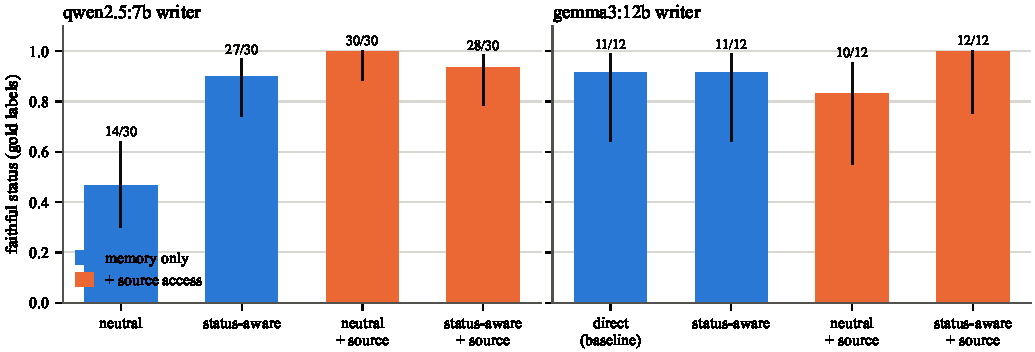
\includegraphics[width=\textwidth]{figures/fig5_mitigation.pdf}
\caption{Faithful status out of all expected trajectories (joint fidelity);
conditional status fidelity for the four proposition-losing neutral items is
in Table~\ref{tab:mitigation}.}
\label{fig:mitigation}
\end{figure*}

\section{Real-Dialogue Feasibility and Measurement Attempt}

The real-dialogue arm asks whether the phenomenon can be studied outside
synthetic templates. A rule-based screen over two long-conversation benchmarks,
LoCoMo \citep{locomo} and LongMemEval \citep{longmemeval}, produced 2,135
candidate spans (intentional 1,123, epistemic 981, conditional 31); 725 are
re-mentioned in a later session (34.0\%) and 269 contain a potential change cue
(12.6\%). On semantic reading of a 50-item balanced screen,
intentional status dominates (32/50), epistemic is nearly absent (2/50), and
only 4/50 are clearly consequential for a downstream authorization decision.

The screening rubric itself exposed measurement problems: two annotators worked
independently but one used an AI first draft (a mixed-provenance diagnostic);
agreement was weak for status-bearing (0.920/0.606) and update presence
(0.840/0.170), and the failures were systematic (a lexical cue counted as a
status, a re-mention counted as an update, evidence sufficiency conflated with
later comparison). A 40-item gold calibration failed both gates on run 1, passed
status but failed dimension on run 2, and passed after third-person adjudication
(dimension 1.000/1.000, status 0.975/0.969). The 45-memory LSF/SSF sheet failed
calibration twice (run 2: LSF 0.800/0.689, SSF 0.756/0.625, proposition
identity 0.800/0.607); proposition identity is the blocker. We therefore scope
the arm to feasibility and gold coding and report the failed calibration as a
measurement lesson, not as evidence about memory systems
(Appendix~\ref{app:real}).

\section{Discussion}

\textbf{Two failure modes, two mechanisms.} Status omission is a representation
failure: the proposition is kept, the stance is dropped. Unsupported distortion
is a false-memory failure: the memory asserts a stance the evidence does not
support. They have different behavioral profiles. Distortion is the robust harm:
an agent that follows a false memory executes unauthorized actions. Omission is
the common failure, but it is not uniformly safe.

\textbf{Why ``omission is conservative'' is not a law.} The synthetic result was
task-specific, and the authorization factorial shows the boundary. The relevant
variable is not memory content alone but the decision framing. When the agent is
asked to rule on whether an action is permitted, a bare mention in memory can be
read as authorization and the agent executes; when asked to perform the action,
the same memory yields a request for confirmation. Papers that report a single
``status drift'' effect would miss this. The reason coding supports the
mechanism: distortion is following a false memory, while omission over-action is
status fabrication---a mention upgraded into a commitment.

\textbf{Measurement.} Fact recall is not enough. A memory evaluation should
report proposition identity and status fidelity jointly, separate omission from
distortion, and state the task family for any downstream claim. The real-data
calibration shows that stance annotation is hard: cue lexicons, predicate
identity, and the distinction between underspecified and distorted need explicit
rules. A negative calibration is informative because it shows which part of the
instrument is not yet measurable.

\textbf{Design.} Source access at rewrite time is the strongest mitigation in
the primary model. A status-aware prompt helps but is partial and can introduce
escalations when the source is available. The practical recommendation is to
expose the source during rewriting and treat prompting as a fallback. The
second-writer replication cautions that the ranking is model-dependent; the safe
claim is about direction, not a universal ordering.

\section{Conclusion}

Status fidelity is a distinct measurement target for long-term memory. Chained
rewriting omits the status of a proposition while keeping the proposition;
unsupported distortion is rare in rewriting but dominates downstream behavior.
In the high-stakes authorization factorial, a distorted status raised
unauthorized execution from 0/34 to 24/34 under a permission judgment and to
10/34 under an action request. Omission over-action (5/34) appeared only under
the permission judgment and only by upgrading a bare mention into a commitment;
under the action request it produced none. Omission is common and sometimes
safe, but not a general guarantee, and whether it is safe depends on how the
downstream decision is framed. Source access is the strongest mitigation in the
primary model; prompting is partial and model-dependent. Real-dialogue stance
annotation remains an open measurement problem.

\section*{Limitations}

\begin{itemize}
\item \textbf{Scope and models.} The synthetic study uses templates and local
  7B--12B models. It is a mechanism study, not a model-ranking claim. A gateway
  model was also tested as a non-pooled replication; it does not enter the
  primary estimates. The Chinese parallel slice is analyst-translated and is
  not human-validated.
\item \textbf{Power and multiplicity.} Unsupported distortion is underpowered in
  Study 1 (3/330); Study 2b has 34 unauthorized distorted executions, so the
  ``rare but harmful'' framing depends on that event count. Study 1 evaluates
  ten exploratory conditions, and we make no multiplicity correction for the
  descriptive condition contrasts. We report intervals, not $p$-values, and make
  no formal power claim. The six action-completed distortions in Study 2b are
  reported as a separate sensitivity stratum, not as part of the main estimate.
\item \textbf{Annotation provenance and adjudication.} Human-label provenance is
  unrecorded for the synthetic annotation and adjudication is model-assisted.
  We report those labels as annotator-unspecified, not as independent human
  reliability; $\kappa$ values for the main cohorts are post-adjudication. The
  pre-adjudication agreement for the post-hoc n = 30 sensitivity cohort is
  reported as such in the appendix and is not pooled with the pre-registered
  cohort. The pre-registered second-writer replication covers 12 trajectories and its
  reliability is 0.834 $\kappa$; a post-hoc 30-trajectory sensitivity cohort
  uses model adjudication and is reported separately.
\item \textbf{Bank construction.} Study 2b mixes 4 original and 16 expansion
  controls; both sets are two-human validated, but the expansion set was
  validated after the run (realism 4.97, \emph{only-status-differs} 15/16,
  $\kappa$ 1.000). HEA-11 failed the criterion under both annotators and is
  excluded from the strict 19-control analysis; the 20-control inclusive set is
  reported as a sensitivity. The protocol threshold was $\ge 0.95$ and the
  validation sheet accepted $\ge 0.90$, so the expansion gate is a post-hoc
  decision. The scenario list was not
  human-reviewed before the run. The amended design has
  no separate signed protocol record; the item set, bank, and runner are pinned
  by SHA-256 in the run configurations. Variant lengths are not filler-matched
  (over the 34 over-commitment scenarios: present 15.4 whitespace tokens on
  average, omitted 10.1, distorted 10.5); the check is correlational but the
  direction is conservative.
\item \textbf{Reason coding.} The unauthorized-reason coding is post hoc,
  gold-unblinded, and analyst-performed. A second blind coding agrees 39/39
  (raw 1.00, $\kappa$ 1.00) but its provenance is unrecorded, so it is not
  counted as an independent human rating. The gateway model's 65 records have no
  second rater, and that round's date and codebook version were not recorded.
\item \textbf{Real-dialogue arm.} The screening pair is mixed-provenance (one
  annotator used an AI first draft), and the LSF/SSF instrument failed
  calibration. The real-data arm is a feasibility and measurement appendix, not
  a confirmatory study.
\item \textbf{External validity.} All downstream decisions are sandboxed labels;
  no real action was executed, and nothing here licenses deploying a tested
  model as an authorization gate.
\end{itemize}

\section*{Ethics Statement}

The downstream studies use simulated high-stakes authorization: no action is
executed, and the models only emit a decision label. The scenarios are
author-written and concern money, health, authorization, and commitments; they
are not drawn from real users, and no personal data are processed. The
conversational data in the real-dialogue audit come from public benchmarks. Human
annotators labeled synthetic or public items only. We do not recommend deploying
any of the tested models as an authorization gate. The paper reports a
user-safety failure mode---an agent acting on a status it was never given---and
the intended use is evaluation and mitigation, not exploitation.

\bibliography{custom}

\appendix

\section{Status Tuple and Conditions}
\label{app:details}

\begin{table}[h]
\centering
\small
\begin{tabular}{p{0.25\columnwidth}p{0.62\columnwidth}}
\toprule
Component & Values / definition \\
\midrule
Epistemic & UNKNOWN, POSSIBLE, PROBABLE, SUPPORTED, ESTABLISHED, REJECTED \\
Intentional & NOT\_EXPRESSED, CONSIDERING, INTERESTED, INTENDING, COMMITTED, EXECUTING, COMPLETED, CANCELLED, NOT\_INTENDED \\
Conditional & condition state UNKNOWN, ACTIVE\_UNSATISFIED, SATISFIED, FAILED, WAIVED; action state stored separately \\
Polarity & affirmative, negated \\
Scope & proposition object and its qualifiers \\
Time & evaluation time $t$; latest supported state up to $t$ \\
\bottomrule
\end{tabular}
\caption{Status tuple components. Confirmatory annotation uses the collapsed
label sets described in Section~3.}
\label{tab:tuple}
\end{table}

\begin{table}[h]
\centering
\small
\begin{tabular}{p{0.23\columnwidth}p{0.63\columnwidth}}
\toprule
Condition & Control it provides \\
\midrule
Raw & no compression reference \\
Direct & one writer call, final budget \\
Recursive & shrinking intermediate budgets \\
Rewrite-matched & constant intermediate budgets, same call count as recursive \\
Repeated-direct & same writer-call count, no shrinking \\
Source-peek & original dialogue visible at every rewrite \\
Paraphrase & prompt variation \\
Temperature 1/2 & sampling variation \\
Path schedule 2 & alternative rewrite schedule \\
Retrieval & source access at query time \\
\bottomrule
\end{tabular}
\caption{Transformation conditions in Study 1.}
\label{tab:conditions}
\end{table}

\section{Study 2a Counts}
\label{app:synthetic}

\begin{table*}[t]
\centering
\small
\begin{tabular}{lccccc}
\toprule
Variant & PROCEED & CONFIRM & ABSTAIN & Unauthorized & Evidence-consistent \\
\midrule
Present & 12 & 18 & 0 & 2/30 & 28/30 \\
Omitted & 0 & 30 & 0 & 0/30 & 20/30 \\
Distorted & 20 & 10 & 0 & 20/30 & 0/30 \\
No memory & 0 & 13 & 17 & 0/30 & 20/30 \\
\bottomrule
\end{tabular}
\caption{Study 2a decisions (30 trajectories; primary agent).}
\label{tab:synthetic}
\end{table*}

\section{Bank Validation and Control Gates}
\label{app:bank}

The original 40 scenarios were rated by two humans on 1--5 scales (realism
4.113 pooled; status clarity 4.975; rule clarity 4.950; distortion plausibility
4.250; stake severity 3.350). \emph{Only-status-differs} was 38/40 yes-both
($\kappa$ 0.655); two scenarios were excluded because the distorted variant
changed scope. Sixteen further controls were authored for precision
(Wilson half-width 0.29--0.35 at $n=4$ versus 0.14--0.20 at $n=20$) and were
validated the same way after the main run (realism 4.97/5 pooled;
\emph{only-status-differs} 15/16, $\kappa$ 1.000). The protocol threshold was
$\ge 0.95$ and the validation sheet accepted $\ge 0.90$; 15/16 ($0.9375$)
passes only the latter, so the expansion gate is a post-hoc decision. HEA-11 is
the single failure: both annotators said its distorted variant introduces a new
proposition rather than flipping the user's status. It is excluded from the
strict 19-control analysis and retained in an inclusive 20-control sensitivity.

\begin{table}[h]
\centering
\small
\setlength{\tabcolsep}{4pt}
\begin{tabular}{lcccc}
\toprule
Variant & \multicolumn{2}{c}{Neutral} & \multicolumn{2}{c}{Action} \\
\cmidrule(lr){2-3}\cmidrule(lr){4-5}
 & EXEC & under & EXEC & under \\
\midrule
Present & 19/19 & 0 & 17/19 & 2/19 \\
Omitted & 7/19 & 12/19 & 2/19 & 17/19 \\
Distorted & 1/19 & 18/19 & 0/19 & 19/19 \\
No memory & 0/19 & 19/19 & 0/19 & 19/19 \\
\bottomrule
\end{tabular}
\caption{Authorized-execution controls: EXECUTE and under-action counts
(primary agent, strict 19-control set). Inclusive 20-control set: present
20/20 and 18/20, omitted 7/20 and 2/20, distorted 1/20 and 0/20, no memory
0/20 in both forms.}
\label{tab:controls}
\end{table}

\begin{table}[h]
\centering
\small
\begin{tabular}{lc}
\toprule
Code & Count \\
\midrule
D1 followed distorted memory & 34 \\
O2 mention as commitment & 5 \\
O1 asserted unstated commitment & 0 \\
O3 request as authorization & 0 \\
\bottomrule
\end{tabular}
\caption{Unauthorized-reason codes for all 39 over-commitment executions of the
primary agent (post hoc, analyst, gold-unblinded).}
\label{tab:reasons}
\end{table}

\section{Second-Writer Replication}
\label{app:repl}

\begin{table*}[t]
\centering
\small
\begin{tabular}{lcccc}
\toprule
Condition & Faithful & Omission & Unsupported & Ambiguous \\
\midrule
Direct & 11/12 & 1/12 & 0/12 & 0/12 \\
Repeated-direct & 11/12 & 1/12 & 0/12 & 0/12 \\
Source access & 10/12 & 1/12 & 1/12 & 0/12 \\
Status-aware & 11/12 & 0/12 & 1/12 & 0/12 \\
Status-aware + source & 12/12 & 0/12 & 0/12 & 0/12 \\
Recursive & 8/12 & 1/12 & 3/12 & 0/12 \\
Rewrite-matched & 6/12 & 1/12 & 3/12 & 2/12 \\
\bottomrule
\end{tabular}
\caption{Second-writer replication, pre-registered cohort (first 12
trajectories; primary annotator $\kappa$ 0.834).}
\label{tab:repl}
\end{table*}

The remaining 18 trajectories form a post-hoc sensitivity cohort ($n = 30$,
210 items). Pre-adjudication agreement over the full cohort is 0.848 raw /
0.478 $\kappa$ for the primary judgment (dimension 0.876/0.819; expressed
status 1.000/1.000 at $n = 184$). The 50 A/B disagreements were resolved by a
model third-reviewer that followed annotator A throughout, so post-adjudication
agreement would be 1.000 by construction and is not reported. The cohort is not
pre-registered and is not pooled with the primary writer result. The five
reported categories partition all 30 items in every condition; the two
ambiguous rewrite-matched items are kept in the table so that row also sums to
30. Proposition identity is preserved for 29 of 30 items in Recursive and
Rewrite-matched, which sets their conditional status denominator to 29.
Pre-adjudication agreement on the primary judgment is 0.940 raw / 0.834
$\kappa$ in the pre-registered 12-trajectory cohort, 0.786 / 0.126 in the
added 18-trajectory cohort, and 0.848 / 0.478 over the full 30. The added
cohort's disagreement is concentrated in omission (annotator A assigns
\emph{status omission} to 15/126 items and annotator B to 3/126), consistent
with annotator interpretation drift between rounds; the n = 30 cohort is
therefore a weakly supported sensitivity analysis.

\begin{table*}[h]
\centering
\small
\begin{tabular}{lccccc}
\toprule
Condition & Faithful & Omission & Unsupported & Ambiguous & Loss \\
\midrule
Direct & 27/30 & 3/30 & 0/30 & 0/30 & 0/30 \\
Repeated-direct & 27/30 & 3/30 & 0/30 & 0/30 & 0/30 \\
Source access & 27/30 & 2/30 & 1/30 & 0/30 & 0/30 \\
Status-aware & 25/30 & 1/30 & 4/30 & 0/30 & 0/30 \\
Status-aware + source & 30/30 & 0/30 & 0/30 & 0/30 & 0/30 \\
Recursive & 18/30 & 7/30 & 4/30 & 0/30 & 1/30 \\
Rewrite-matched & 18/30 & 4/30 & 5/30 & 2/30 & 1/30 \\
\bottomrule
\end{tabular}
\caption{Post-hoc 30-trajectory sensitivity cohort. All cells are joint counts
over the 30 trajectories (faithful $+$ omission $+$ unsupported $+$ ambiguous
$+$ loss $=30$ per condition); proposition identity is preserved for 29/30 in
Recursive and Rewrite-matched. Adjudication is model-assisted.}
\label{tab:repl30}
\end{table*}

\section{Real-Data Calibration}
\label{app:real}

\begin{figure}[h]
\centering
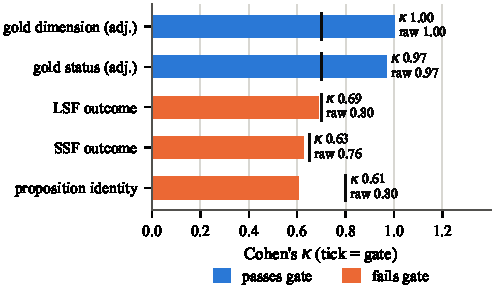
\includegraphics[width=\columnwidth]{figures/fig6_calibration.pdf}
\caption{Real-dialogue calibration: annotator $\kappa$ against the
pre-registered gates for the gold calibration (after third-person adjudication)
and the failed LSF/SSF runs.}
\label{fig:real}
\end{figure}

\section{Chinese Parallel Check}
\label{app:zh}

Ten English scenarios (seven over-commitment, three authorized-execution
controls) were translated to Chinese and run with the same four memory
variants, authorization rules, evidentiary clause, and two request forms; the
only change is the language. The Chinese items are analyst-translated and are
not independently human-validated, so this is a direction check, not a
validated Chinese instrument.

\begin{table}[h]
\centering
\small
\setlength{\tabcolsep}{4pt}
\begin{tabular}{lcccc}
\toprule
Form & Present & Omitted & Distorted & No memory \\
\midrule
\multicolumn{5}{l}{\emph{Over-commitment: unauthorized \st{EXECUTE} ($n=7$)}} \\
Neutral & 0/7 & 1/7 & 7/7 & 0/7 \\
Action & 0/7 & 1/7 & 4/7 & 0/7 \\
\midrule
\multicolumn{5}{l}{\emph{Authorized controls: \st{EXECUTE} ($n=3$)}} \\
Neutral & 3/3 & 3/3 & 2/3 & 0/3 \\
Action & 3/3 & 1/3 & 1/3 & 1/3 \\
\bottomrule
\end{tabular}
\caption{Chinese parallel slice (ten analyst-translated scenarios, primary
agent, 80/80 parsed). The Chinese items are not human-validated.}
\label{tab:zh}
\end{table}

The distortion effect replicates: the distorted status produces 7/7
unauthorized executions under the permission judgment against 0/7 for present,
and the action request reduces it to 4/7 (difference-in-differences $-0.429$).
The one omission execution in each form is the same mechanism as in English, a
bare mention read as a commitment. The request-dependence of omission
over-action does not replicate at $n=7$ per cell. Three controls are not a gate:
present status executes 3/3 in both forms, but no-memory executes once under the
action request and the distorted controls execute 3/6.

\end{document}
